\documentclass[aspectratio=169,UTF8,zihao=-4]{ctexbeamer}

\usetheme{Madrid}
\usecolortheme{default}
\setbeamertemplate{navigation symbols}{}
\setbeamertemplate{headline}{}
\setbeamertemplate{frametitle}{}
\setbeamertemplate{footline}[frame number]

\usepackage{amsmath}
\usepackage{booktabs}
\usepackage{array}
\usepackage{graphicx}
\graphicspath{{./}}

\IfFontExistsTF{Sarasa Gothic SC}{
  \setCJKmainfont[AutoFakeBold=2.5]{Sarasa Gothic SC}
  \setCJKsansfont[AutoFakeBold=2.5]{Sarasa Gothic SC}
  \setCJKmonofont{Sarasa Mono SC}
}{}

\title{小优惠也能撬动消费？}
\subtitle{优惠券面额与使用门槛对消费兑现意愿的影响}
\author{第6组：程乾坤、雷佑宁、刘欣悦、刘子溱、王鲲淏、章玉树}
\date{\today}

\newcommand{\bigidea}[1]{
  \begin{center}
    \vspace{0.8em}
    {\LARGE \bfseries #1}
    \vspace{0.6em}
  \end{center}
}

\newcommand{\sectionpageframe}[1]{
  \begin{frame}[plain]
    \begin{center}
      \vfill
      {\Huge \bfseries #1}
      \vfill
    \end{center}
  \end{frame}
}

\begin{document}

\begin{frame}[plain]
  \titlepage
\end{frame}

\sectionpageframe{一、变量名称及其定义}

\begin{frame}
  \begin{itemize}
    \item \Large 自变量1：优惠券面额
    \item \Large 自变量2：使用门槛
    \item \Large 因变量：消费兑现意愿
  \end{itemize}
\end{frame}

\begin{frame}
  \bigidea{优惠券面额}
  \begin{itemize}
    \item \Large 优惠券可直接减免的金额
    \item \Large “满100减10”中的10元
    \item \Large 本研究设置为 5 元 vs. 25 元
  \end{itemize}
\end{frame}

\begin{frame}
  \bigidea{使用门槛}
  \begin{itemize}
    \item \Large 优惠券生效前必须达到的最低消费额
    \item \Large “满X元可用”中的X元
    \item \Large 本研究设置为无门槛、满30元、满80元
  \end{itemize}
\end{frame}

\begin{frame}
  \bigidea{消费兑现意愿}
  \begin{itemize}
    \item \Large 消费者实际使用优惠券并完成消费的主观倾向
    \item \Large "我愿意使用该优惠券进行消费"
    \item \Large 使用 7 点 Likert 量表测量
  \end{itemize}
\end{frame}

\sectionpageframe{二、假设的完整陈述}

\begin{frame}
  \bigidea{H1：面额的正向作用}
  \begin{itemize}
    \item \Large 高面额推动消费者支出水平
    \item \Large 大额面额能够显著提升促销的吸引力
    \item \Large 数字优惠券影响消费者兑现意愿
  \end{itemize}
\end{frame}

\begin{frame}
  \bigidea{H2：门槛的负向作用}
  \begin{itemize}
    \item \Large 门槛约束提升消费者的购买概率和购买量
    \item \Large 过高的门槛降低兑现意愿
    \item \Large 消费者进行"门槛努力—面额收益"的成本收益分析
    \item \Large 消费门槛较高，难以将优惠券与具体消费需求匹配，兑现意愿大幅弱化
  \end{itemize}
\end{frame}

\begin{frame}
  \bigidea{H3：面额与门槛的交互}
  \begin{itemize}
    \item \Large 门槛较低时，优惠券面额对消费兑现意愿的正向影响更强
    \item \Large 使用门槛较高时，优惠券面额的正向影响会显著减弱，甚至趋于不显著
    \item \Large 消费者高努力感知会显著削弱面额的正向作用
  \end{itemize}
\end{frame}

\sectionpageframe{三、模型的图示}

\begin{frame}
  \centering
  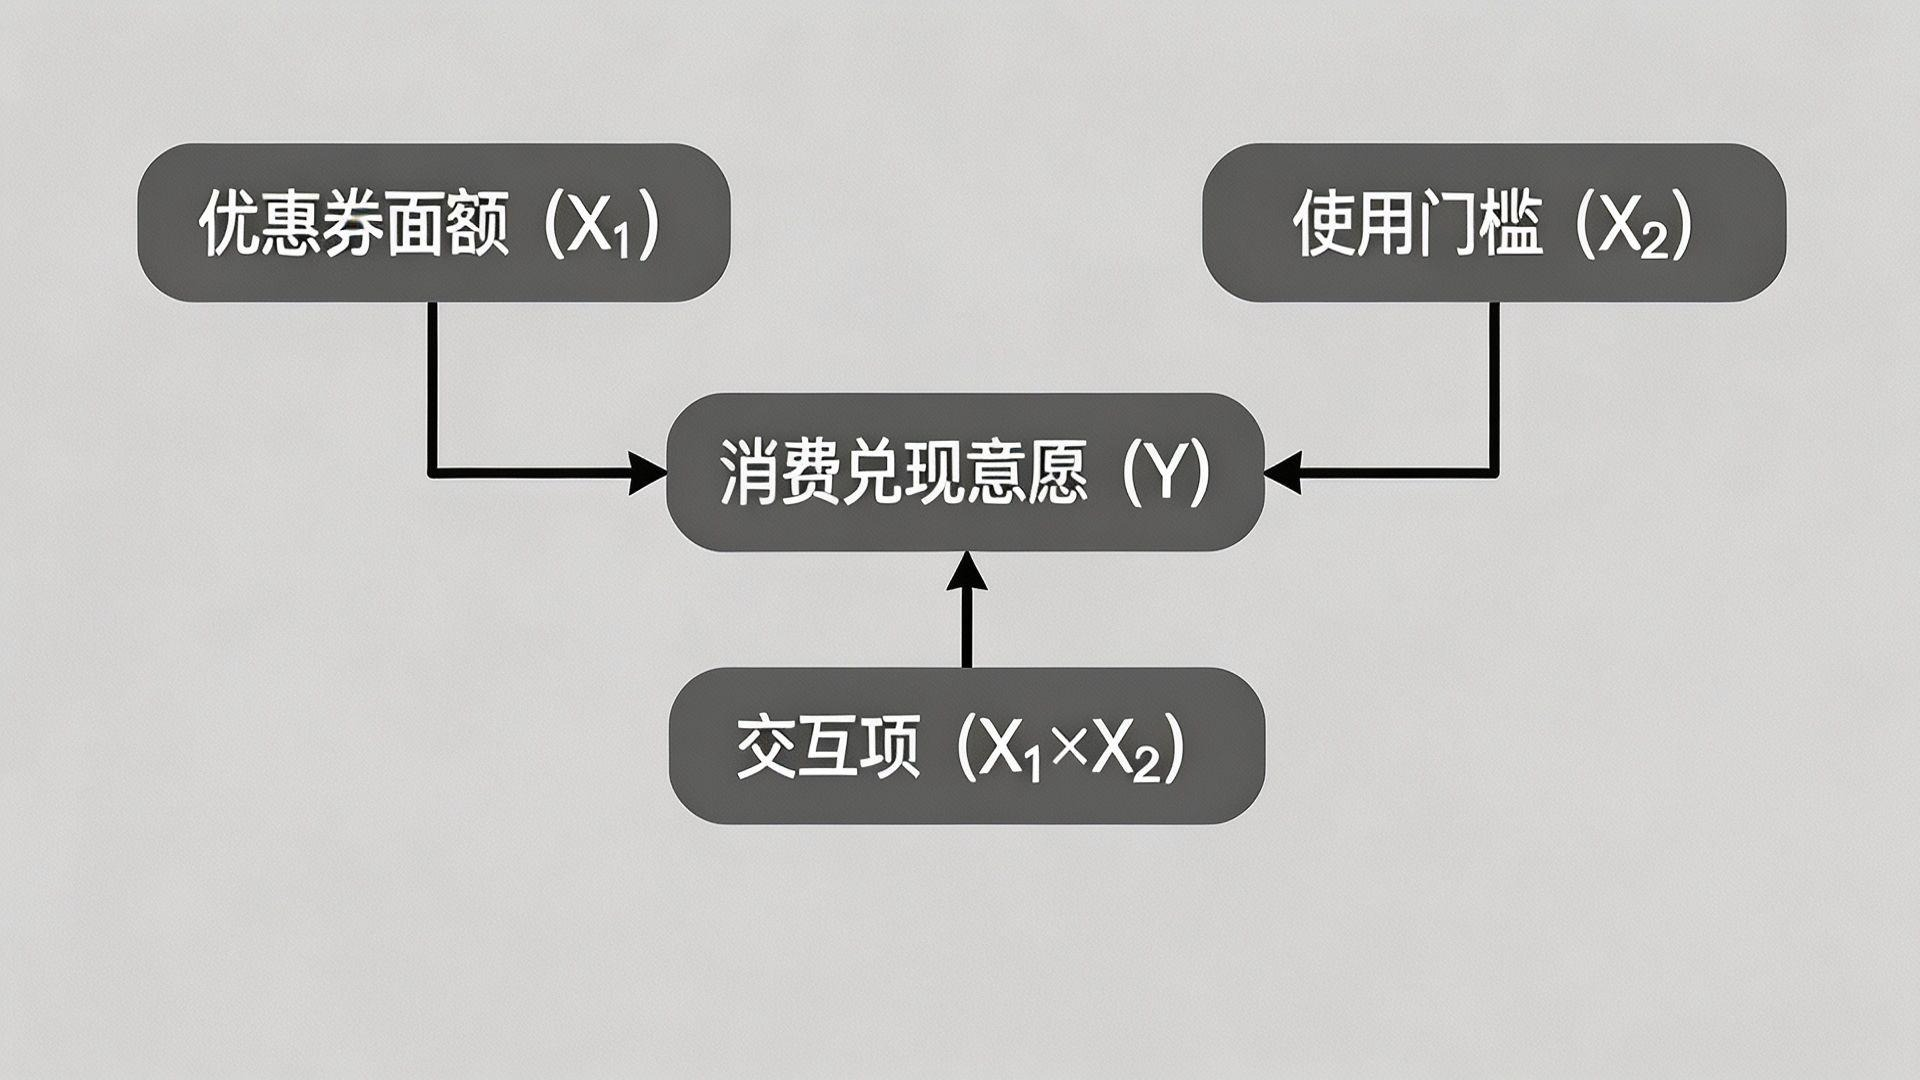
\includegraphics[width=0.76\textwidth,height=0.55\textheight,keepaspectratio]{group6_experiment_model.jpeg}

\end{frame}

\begin{frame}
  \bigidea{$2 \times 3$ 被试间实验}
  \centering
  \Large
  \setlength{\tabcolsep}{7pt}
  \begin{tabular}{lll}
    \toprule
    实验因素 & 水平数 & 具体水平 \\
    \midrule
    优惠券面额 & 2个水平 & 5元、25元 \\
    使用门槛 & 3个水平 & 无门槛、满30元、满80元 \\
    \bottomrule
  \end{tabular}

  \vspace{1.2em}
  \begin{itemize}
    \item \Large 计划样本量约 180 人，每组约 30 人
  \end{itemize}
\end{frame}

\sectionpageframe{五、自变量的操控方法和检验方法}

\begin{frame}
  \bigidea{文字情景模拟}
  \begin{itemize}
    \item \Large 可以从外部操控实验因素的水平，保证高内部效度
    \item \Large 标准化实验条件，消除无关变量的干扰
  \end{itemize}
\end{frame}

\begin{frame}
  \begin{itemize}
    \item \Large 你是一名在校大学生，平时经常购买咖啡或茶饮。某天，你在手机上收到一张来自"悦享咖啡"的电子优惠券。"悦享咖啡"是一家全国连锁的咖啡茶饮品牌（为实验需要虚构，非真实品牌），在学校周边设有门店，支持到店取餐和外送服务。该品牌的定价与瑞幸咖啡、库迪咖啡等常见大学生消费品牌相当：标准饮品（美式、拿铁等）单价约15-25元，轻食（三明治、烘焙等）单价约20-35元。优惠券有效期为7天。
  \end{itemize}
\end{frame}

\begin{frame}
  \bigidea{自变量操控}
  \begin{columns}[T]
    \column{0.48\textwidth}
    \begin{block}{面额}
      \Large
      低面额：5元\\
      高面额：25元\\
      25元约等于一杯饮品
    \end{block}
    \column{0.48\textwidth}
    \begin{block}{门槛}
      \Large
      无门槛\\
      满30元\\
      满80元
    \end{block}
  \end{columns}
\end{frame}

\begin{frame}
  \bigidea{预测试}
  \begin{itemize}
    \item \Large 招募 15--20 名不参加正式实验的被试
    \item \Large 随机分配到 6 个实验组
    \item \Large 面额识别：优惠金额是 5 元还是 25 元
    \item \Large 门槛识别：无门槛、满30元还是满80元
    \item \Large 情景真实感：是否贴近真实咖啡消费
  \end{itemize}
\end{frame}

\sectionpageframe{六、实验流程设计}

\begin{frame}
  \bigidea{被试获取}
  \begin{itemize}
    \item \Large 本科生和研究生，18--28岁
    \item \Large 过去一个月买过咖啡或茶饮
    \item \Large 有过优惠券使用经验
    \item \Large 通过校园微信群、朋友圈、班级群和线下海报招募
  \end{itemize}
\end{frame}

\begin{frame}
  \bigidea{样本量}
  \begin{itemize}
    \item \Large 6 个实验组，每组约 30 人
    \item \Large 中等效应量 $f=0.25$
    \item \Large 显著性水平 0.05，统计功效 0.80
    \item \Large 最低样本量约 158 人
    \item \Large 考虑无效问卷后计划回收约 180--186 份
  \end{itemize}
\end{frame}

\begin{frame}
  \bigidea{问卷结构}
  \centering
  \large
  \setlength{\tabcolsep}{6pt}
  \begin{tabular}{lll}
    \toprule
    顺序 & 模块 & 作用 \\
    \midrule
    1 & 筛选题 & 确认目标被试 \\
    2 & 知情同意 & 告知研究与权利 \\
    3 & 情景材料 & 呈现实验操控 \\
    4 & 消费兑现意愿 & 测量因变量 \\
    5 & 混淆变量 & 控制个体差异 \\
    6 & 操控检验 & 检查操控有效性 \\
    7 & 人口统计与解说 & 背景信息与去欺骗 \\
    \bottomrule
  \end{tabular}
\end{frame}

\begin{frame}
  \bigidea{消费兑现意愿问项}
  \begin{itemize}
    \item \Large 我会在有效期内使用这张优惠券
    \item \Large 我愿意为了使用它而专门前往消费
    \item \Large 考虑到优惠券条件，我认为使用它是值得的
    \item \Large 原本没有购买计划时，也可能因此去消费
    \item \Large 与其他促销相比，这张优惠券有吸引力
  \end{itemize}
\end{frame}

\begin{frame}
  \bigidea{质量控制}
  \begin{itemize}
    \item \Large 注意力检查：要求被试选择指定选项
    \item \Large 剔除作答时间低于 2 分钟的问卷
    \item \Large 剔除认真度低于 4 分的问卷
    \item \Large IP 去重，检查开放反馈
    \item \Large 预计剔除 12\%--15\% 的无效样本
  \end{itemize}
\end{frame}

\sectionpageframe{七、预实验设计}

\begin{frame}
  \bigidea{预实验目的}
  \begin{itemize}
    \item \Large 选择最合适的消费品类
    \item \Large 降低品类偏好和品牌偏好的干扰
    \item \Large 检查实验情景是否真实、易懂
    \item \Large 如果咖啡/茶饮不合适，再替换品类和门槛金额
  \end{itemize}
\end{frame}

\begin{frame}
  \bigidea{候选品类}
  \centering
  \large
  \begin{tabular}{lll}
    \toprule
    品类 & 典型场景 & 优势 \\
    \midrule
    咖啡/茶饮 & 校园周边饮品 & 高频、价格清晰 \\
    外卖/简餐 & 平台满减优惠 & 门槛促销常见 \\
    线上超市 & 日用品即时零售 & 商品较标准化 \\
    \bottomrule
  \end{tabular}
\end{frame}

\begin{frame}
  \bigidea{评估维度}
  \begin{itemize}
    \item \Large 熟悉度：是否了解该品类
    \item \Large 优惠券感知：是否认为该品类常见优惠券
    \item \Large 偏好一致性：同学之间偏好差异是否较小
    \item \Large 情景真实性：是否贴近真实生活
    \item \Large 每项采用 1--7 分评分
  \end{itemize}
\end{frame}

\sectionpageframe{八、数据分析计划}

\begin{frame}
  \bigidea{数据清洗}
  \begin{itemize}
    \item \Large 删除筛选题不符合要求的样本
    \item \Large 删除注意力检查失败和认真度过低样本
    \item \Large 计算 5 个 CRI 题项的均值
    \item \Large 检查正态性和方差齐性
  \end{itemize}
\end{frame}

\begin{frame}
  \bigidea{操控检验}
  \begin{itemize}
    \item \Large 面额识别：使用卡方检验
    \item \Large 门槛识别：使用卡方检验
    \item \Large 情景真实感：比较各组均值
    \item \Large 预期面额正确率不低于 90\%
    \item \Large 预期门槛正确率不低于 85\%
  \end{itemize}
\end{frame}

\begin{frame}
  \bigidea{假设检验}
  \begin{block}{核心方法}
    \begin{center}
      {\Large $2 \times 3$ 双因素被试间方差分析}
    \end{center}
  \end{block}
  \begin{itemize}
    \item \Large 面额主效应检验 H1
    \item \Large 门槛主效应检验 H2
    \item \Large 面额 $\times$ 门槛交互项检验 H3
    \item \Large 交互显著时进一步做简单效应分析
  \end{itemize}
\end{frame}

\begin{frame}
  \bigidea{信度与稳健性}
  \begin{itemize}
    \item \Large 对消费兑现意愿量表计算 Cronbach's alpha
    \item \Large $\alpha \ge 0.70$ 视为可接受
    \item \Large 将优惠券倾向性、价格敏感度、情绪和品牌偏好作为协变量
    \item \Large 使用 ANCOVA 检查结论是否稳健
  \end{itemize}
\end{frame}

\begin{frame}
  \bigidea{谢谢大家}
\end{frame}

\end{document}
